\chapter{Reflection}
% \section*{9 - Ottobre}
\section{Introduction and Definitions}

\textbf{Reflection} is the ability of a program to manipulate as data something representing the state of the program during its own execution.
Another dimension of reflection is if a program is
allowed to \textbf{read only}, or also to \textbf{change} itself.
\begin{itemize}
    \item \textbf{Introspection} is the ability of a program to observe and
    therefore reason about its own state
    \item \textbf{Intercession} is the ability for a program to modify its
    own execution state or alter its own interpretation or
    meaning
    \item \textbf{Reification} is the mechanism of encoding execution state into data, which is needed by both \textit{introspection} and \textit{intercession}
\end{itemize}

\ul{\textbf{Structural} reflection}  is concerned with the ability of the \textbf{language} to provide a complete \ul{\textit{reification} of both the \textit{program} executed and its \textit{abstract data types}.}\\
\ul{\textbf{Behavioral} reflection} is concerned instead with the \ul{reification of its\footnote{referred to a \textbf{language}} \textit{semantics} \& \textit{implementation} (processor) and the data and implementation of the \textit{run-time system}}.

\section{Uses and drawbacks}
\subsection{Uses}
\begin{itemize}
    \item \textit{Class Browsers} need to be able to enumerate the number of classes
    \item \textit{Visual Development Environments} can exploit type info available in reflection to aid the developer in writing correct code
    \item \textit{Debuggers} need to be able to examine private members on classes
    \item \textit{Test Tools} exploit reflection to ensure a high level of code coverage in a test suite
    \item \textit{Extensibility Features} an app may make use of external, user-defined classes by creating instances of extensibility objects.
\end{itemize}

\subsection{Drawbacks}
If it is possible to perform an operation without using reflection, then it is
preferable to avoid using it. Reflection is powerful, but it has some drawbacks:
\begin{itemize}
    \item \textbf{Performance Overhead} - Reflection involves types that are dynamically resolved, thus optimizations
    can not be performed, and reflective operations have slower performance
    than their non-reflective counterparts
    \item \textbf{Security Restrictions} - Reflection requires a runtime permission which may not be present when
    running under a security manager. This affects code which has to run in a
    restricted security context, such as in an Applet.
    \item \textbf{Exposure of internals} - Reflective code may access internals (like private fields), thus it breaks
    abstractions and may change behavior with upgrades of the platform,
    destroying portability.
\end{itemize}

\section{Reflection in Java}
Java supports \textbf{introspection} and \textbf{reflexive invocation},
but not \textit{code modification}.

\subsection{Introspection}

\begin{paracol}{2}
    \colfill
    {The JVM mantains for every type an associated object of type \lstinline{java.lang.Class} which "\textit{reflects}" the type it represents,
    acting as entry point for reflection,
    since it provides all info needed:\ns
    \begin{itemize}
        \item Class name and modifiers
        \item Extended superclasses and implemented inferfaces
        \item Methods, fields, constructors, etc.
    \end{itemize}
    }
    \colfill

    \switchcolumn

    \begin{figure}[htbp]
        \centering
        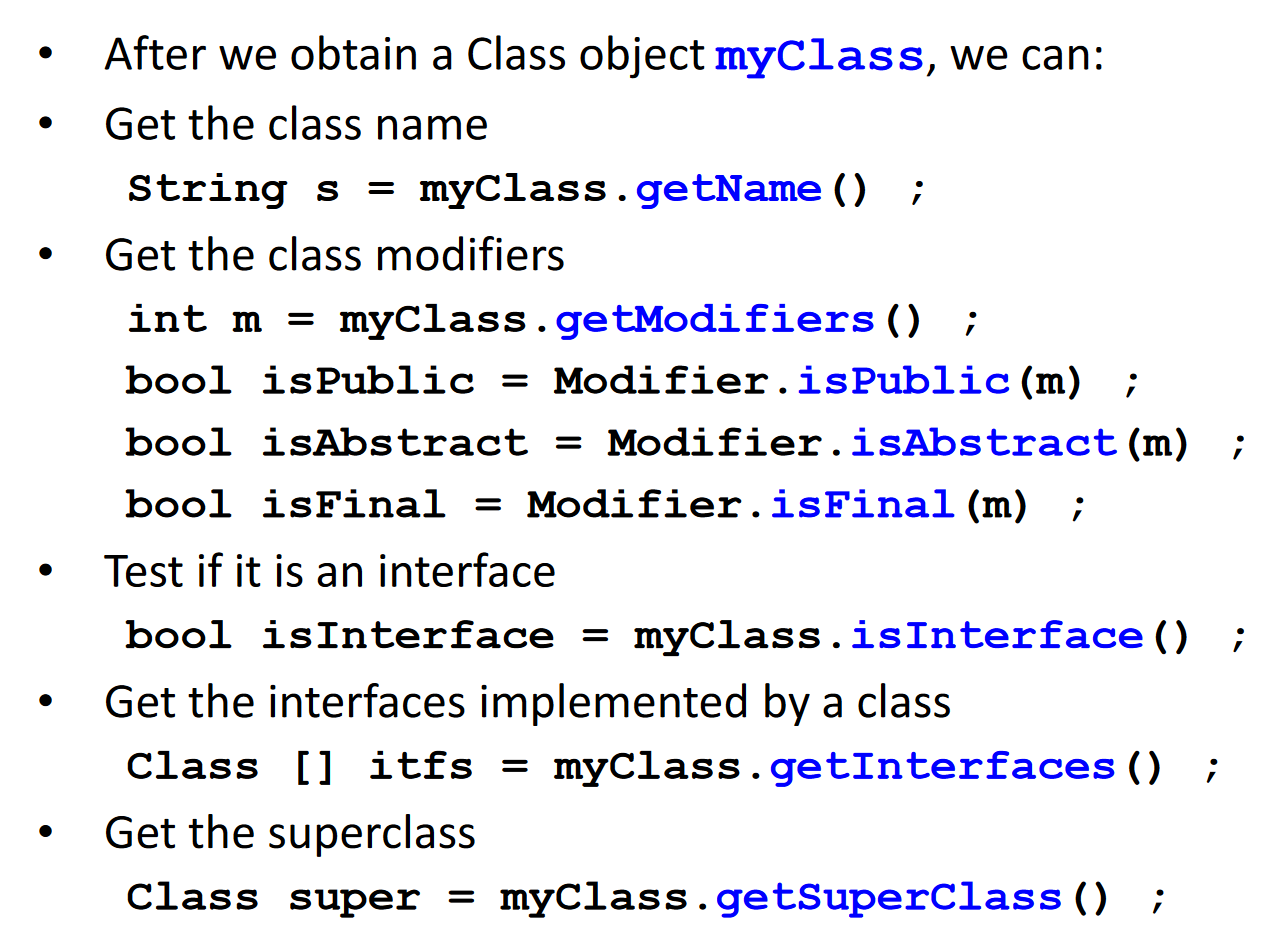
\includegraphics{images/reflection_class.png}
        \caption{Inspecting a Class}
        \label{fig:reflection_class}
    \end{figure}

\end{paracol}

To retrieve such \lstinline{java.lang.Class} object it is sufficient to do \lstinline{Object.getClass()}.
\lstinline{Class} objects are constructed automatically by the JVM as classes are loaded.

Using \lstinline{java.util.reflect.*} it is possible also to retrieve class \textbf{Members} i.e. \textit{fields, constructors} and \textit{methods}.
The extensive \lstinline{java.util.reflect.*} API provides many \textit{methods} to achieve this which will not be reported here.\\
There is a class for each \texttt{Member}
\begin{itemize}
    \item \lstinline{java.util.reflect.Field}: access type info and set/get values.
    \item \lstinline{java.util.reflect.Method}: type info for parameters and return type;
    invoking method on a given object.
    \item \lstinline{java.util.reflect.Constructor}: note that constructors have no return values and invocation creates a new instance of the given class.
\end{itemize}


\begin{table}[htbp]
\centering
\begin{tabular}{|c|c|c|c|c|}
\hline
\textbf{Member} & \textbf{Class API} & \textbf{List of members?} & \textbf{Inherited members?} & \textbf{Private members?} \\
\hline
\multirow{4}{*}{Field} & \href{https://docs.oracle.com/javase/8/docs/api/java/lang/Class.html#getDeclaredField-java.lang.String-}{\texttt{getDeclaredField(String)}} & no & no & yes \\
 & \href{https://docs.oracle.com/javase/8/docs/api/java/lang/Class.html#getField-java.lang.String-}{\texttt{getField(String)}} & no & yes & no \\
 & \href{https://docs.oracle.com/javase/8/docs/api/java/lang/Class.html#getDeclaredFields--}{\texttt{getDeclaredFields()}} & yes & no & yes \\
 & \href{https://docs.oracle.com/javase/8/docs/api/java/lang/Class.html#getFields--}{\texttt{getFields()}} & yes & yes & no \\
\hline
\multirow{4}{*}{Method} & \href{https://docs.oracle.com/javase/8/docs/api/java/lang/Class.html#getDeclaredMethod-java.lang.String-java.lang.Class...-}{\texttt{getDeclaredMethod(...)}} & no & no & yes \\
 & \href{https://docs.oracle.com/javase/8/docs/api/java/lang/Class.html#getMethod-java.lang.String-java.lang.Class...-}{\texttt{getMethod(...)}} & no & yes & no \\
 & \href{https://docs.oracle.com/javase/8/docs/api/java/lang/Class.html#getDeclaredMethods--}{\texttt{getDeclaredMethods()}} & yes & no & yes \\
 & \href{https://docs.oracle.com/javase/8/docs/api/java/lang/Class.html#getMethods--}{\texttt{getMethods()}} & yes & yes & no \\
\hline
\multirow{4}{*}{Constructor} & \href{https://docs.oracle.com/javase/8/docs/api/java/lang/Class.html#getDeclaredConstructor-java.lang.Class...-}{\texttt{getDeclaredConstructor(...)}} & no & N/A & yes \\
 & \href{https://docs.oracle.com/javase/8/docs/api/java/lang/Class.html#getConstructor-java.lang.Class...-}{\texttt{getConstructor(...)}} & no & N/A & no \\
 & \href{https://docs.oracle.com/javase/8/docs/api/java/lang/Class.html#getDeclaredConstructors--}{\texttt{getDeclaredConstructors()}} & yes & N/A & yes \\
 & \href{https://docs.oracle.com/javase/8/docs/api/java/lang/Class.html#getConstructors--}{\texttt{getConstructors()}} & yes & N/A & no \\
\hline
\end{tabular}
\caption{Class API Members}
\label{table:class_api_members}
\end{table}



\subsection{Program Manipulation}
By now we have talked only about \textbf{introspection} in java,
but reflection can be used also to create objects of a type not known at compile time,
or to access members (access fields or invoke methods) unknown at compile time.

{Certain operations are \textbf{forbidden} by privacy rules and fail if invoked through reflection:\ns
\begin{itemize}
	\item Changing a final field
	\item Reading or writing a private field
	\item Invoking a private\dots
\end{itemize}}

However the programmer can request that \texttt{Field}, \texttt{Method}, and
\texttt{Constructor} objects to be ``accessible''.
In this case you can invoke method or access field, even if
inaccessible via privacy rules!
\lstinline|AccessibleObject| Class is the superclass of \lstinline|Field|,
\lstinline|Method|, and \lstinline|Constructor|
\note{Request granted if no security manager, or if the existing
security manager allows it}

{\lstinline|AccessibleObject| provides the methods:\ns
\begin{itemize}
	\item \lstinline|boolean isAccessible( )| - Gets the value of the accessible flag for this object
	\item \lstinline|void setAccessible(boolean flag)| - Sets the accessible flag for this object to the indicated boolean value.\\
	This makes a private field accessible, preventing from throwing an \lstinline|IllegalAccessException|.
	\item \lstinline|static void setAccessible(AccessibleObject[] array, boolean flag)| - Sets the accessible flag for an array of objects with a single security check
\end{itemize}}

\section{Case of use}
Reflection may be used for \textbf{Unit Testing} to test methods and their result. JUnit is a framework that makes use of reflection to test methods, exploiting constructs similar to the generic driver below, which however use annotations to mark methods to be tested, instead of naming conventions.

\begin{lstlisting}
public static void testDriver( String testClass ) {
    Class c = Class.forName( testClass );
    Object tc = c.newInstance( );
    Method[ ] methods = c.getDeclaredMethods( );

    for( int i = 0; i < methods.length; i++ ) {
    if( methods[ i ].getName( ).startsWith( "test" ) &&
        methods[ i ].getParameterTypes( ).length == 0 )
        methods[ i ].invoke( tc );
    }
}
\end{lstlisting}

\subsection{JUnit}
JUnit is a testing framework for Java, created by Erich Gamma and Kent Beck.
The \textbf{annotations} listed below are used to mark methods that need to be tested, while \textbf{assertions} are used to verify the correctness of the test ---even one failed \lstinline|assert| and the test fails---, and \textbf{Test Runners} are used to run the tests.

\begin{itemize}
    \item \lstinline|@Test| - Marks a method as a test method.
    \item \lstinline|@Before| - Executed before each test.
    \item \lstinline|@After| - Executed after each test.
    \item \lstinline|@BeforeClass| - Executed once, before the start of all tests.
    \item \lstinline|@AfterClass| - Executed once, after all tests have been finished.
\end{itemize}

\begin{paracol}{2}
    
    \begin{lstlisting}{caption={JUnit will use reflection to find methods annotated and execute them}}
public class ExampleTest {
    @Before
    public void setUp() {
        // Code to set up test environment
    }

    @Test
    public void testSomething() {
        // Test code
    }

    @After
    public void tearDown() {
        // Code to clean up after test
    }
}
    \end{lstlisting}
    
    
    \switchcolumn
    \begin{lstlisting}[basicstyle=\footnotesize\ttfamily]
import java.lang.reflect.Method;
public class SimpleJUnitRunner {
 public static void main(String[] args) throws Exception {
  Class<?> testClass = ExampleTest.class;
  Object testInstance = testClass.getDeclaredConstructor().newInstance();

  Method setUpMethod = null;
  Method tearDownMethod = null;

  for (Method method : testClass.getDeclaredMethods()) {
   if (method.isAnnotationPresent(Before.class)) {
    setUpMethod = method;
   } else if (method.isAnnotationPresent(After.class)) {
    tearDownMethod = method;
   } else if (method.isAnnotationPresent(Test.class)) {
    if (setUpMethod != null) {
     setUpMethod.invoke(testInstance);
    }

    method.invoke(testInstance);

    if (tearDownMethod != null) {
     tearDownMethod.invoke(testInstance);
    }
   }
  }
 }
}
    \end{lstlisting}
\end{paracol}
